
\section{Exercises}
\label{subsec:hydraulics:exercises}
  
\subsection*{Pelton turbine}
\label{subsec:hydraulics:exercises:pelton}

\begin{figure}[!h]
  \centering
  \begin{subfigure}{0.49\textwidth}
    \center
    \includegraphics[width=0.8\textwidth]{pelton.png}
    \caption{Pelton turbine installation}
  \end{subfigure}
  \begin{subfigure}{0.49\textwidth}
    \center
    \includegraphics[width=0.8\textwidth]{peltonSpoon.png}
    \caption{Simplified 2D spoon}
  \end{subfigure}
  \caption{Pelton turbine}
\end{figure}

Consider a two-dimensional jet with flow rate $\vFlow$ and height
impacting a Pelton turbine spoon. The jet is split and the liquid
leaves the spoon in an upper and lower jet, both at an angle of
$\alpha$ with the axial direction. Assume that during the deviation of
the jet, no pressure losses are encountered. Then first for the case
at rest and then for a generic velocity $v_s$ of the spoon:
\begin{itemize}
\item determine the relative and absolute velocity in the jet leaving
  the spoon considering the conservation of total energy in the
  relative frame;
\item compute the force on the spoon;
\item compute the power generated by the turbine and verify the energy
  balance;
\end{itemize}

\clearpage
\subsection*{Aircraft propulsion}
\label{exercise:thrush1}


\begin{figure}[!h]
  \centering
  \includegraphics[width=0.5\textwidth]{thrush.png}
  \caption{Thrush 510G aircraft}
  \label{fig:thrush}
\end{figure}

The Thrush 510G is a small aircraft, equipped with NACA4412 profile
wings with total area of 33.9 $m^2$, whereas the chord is 220 cm. The
cruising speed is 180km/h and the design weight 4800 kg.
\begin{enumerate}
\item Compute the airfoil operating point in cruise, by first
  determining the angle of attack and then the corresponding drag
  force. 
\item The aircraft is powered by a single propeller with a diameter of
  259 cm. Assuming an idealized propeller, what is the homogeneous
  pressure jump over the disk required to maintain speed, if only
  airfoil wing drag needs to be compensated ?
\item Use the Rankine-Froude theorem from section
  \ref{sec:rankineFroude} to determine the energy given to the fluid
  and determine the propulsive efficiency.
\end{enumerate}
Assume standard air at $T=15^\circ C$, \ie $\dens = 1.2257~kg/m^3$ and
$\mu = 1.7965 \times 10^{-5}$.

% \subsection*{Axial pump}

% \begin{itemize}
% \item assuming flow without prerotation ($\aFlowAngle_1 = 0$)
%   determine the stagger angle for a cascade composed of NACA65(8)10
%   blades at solidity $\solidity =1$ for $\flowCoeff=1$ and
%   $\headCoeff=0.5$. 
% \item choose a stator downstream to redress the flow
% \item draw the velocity triangles 
% \item compute total pressure loss
% \item compute reaction coefficient
% \end{itemize}

\clearpage
  
\subsection*{Centrifugal pump}
\label{exercises:pump}

Consider the flow through a centrifugal pump with the following specifications:
\begin{itemize}
\item the working fluid is water, therefore density is constant and
  equal to $\dens = 1000kg/m^3$
\item the blade axial depth in the impeller is uniformly $h_1=h_{2'}=1cm$;
\item at the inlet the radius is $R_{b1}=3cm$, blockage $b_1=0.1$
  and blade angle $\beta_{b1}=-22^\circ$;
\item the outlet radius is $R_{b2}=7.5cm$, blockage $b_2=0.025$ and
  blade angle $\beta_{b2}=-25^\circ$. The flow passage axial depth
  increases to $h_2=2cm$ when moving out of the impeller;
\item the rotational speed is $\rot=3000rpm$ and the volumetric flow
  rate is $\vFlow = 150 m^3/h$.
\end{itemize}
Then 
\begin{enumerate}
\item draw the velocity triangles just before and after entering the
  blades (stations $1$ resp. $1^\prime$) assuming no prewhirl (\ie
  the absolute flow angle $\alpha=0$). Thereby you can assume
  $R_1=R_{1^\prime}=R_{b1}$;
\item Compute the incidence $\delta_1 = \beta_1 - \beta_{b1}$ with
  respect to the blade in the inlet and illustrate these in the
  velocity triangles;
\item draw the velocity triangles just before and after the impeller
  exit (stations $2^\prime$ resp. $2$). Assume perfect guidance in
  the impeller \ie the flow angle $\beta_{2^\prime}$ is the same as
  the blade angle $\beta_{b2}$;
\item compute the total pressure rise, the power and torque of the
  pump.
\end{enumerate}
